%! Author = breandan
%! Date = 2/3/22

% Preamble
\documentclass[11pt]{article}

% Packages
\usepackage{amsmath}
\usepackage{listings}
\usepackage{graphicx}


\lstset{
    basicstyle=\ttfamily,
    columns=fullflexible,
}

\title{COMP 764: High Level Synthesis}
\date{\today}
\author{Breandan Considine}
% Document
\begin{document}
    \maketitle

In our DSL, we consider all variables to be immutable and reassignment will instantiate a phantom instance. Subsequent references will point to the latest instance of the variable, and is denoted using a extra \texttt{'} character in GraphViz. The RTL DSL is untyped and consists of the following operators:

\begin{lstlisting}
         <CONST> ::= 0 | ... | 9 | <CONST> <CONST> | <CONST>.w
           <VAR> ::= RAM | A | ... | Z
            <OP> ::= + | *
          <EXPR> ::= <CONST> | <VAR> | <VAR>[<CONST>] | <EXPR> <OP> <EXPR>
        <MALLOC> ::= <MALLOC>(<CONST>)
     <STATEMENT> ::= <VAR> = <EXPR> | <INDEX> = <EXPR> | <VAR> = <MALLOC>
          <LOOP> ::= for(i in <CONST>..<CONST>) { <STATEMENT> }
\end{lstlisting}

Tests for VHDL generation can be found in:
    
    \texttt{src/jvmTest/kotlin/ai/hypergraph/kaliningraph/vhdl/*}.

\section*{III. VHDL generation}
\subsection*{1. Simple test}

\begin{lstlisting}
RAM = malloc(4);
RAM[3] = RAM[0] * RAM[1] + RAM[2]
\end{lstlisting}

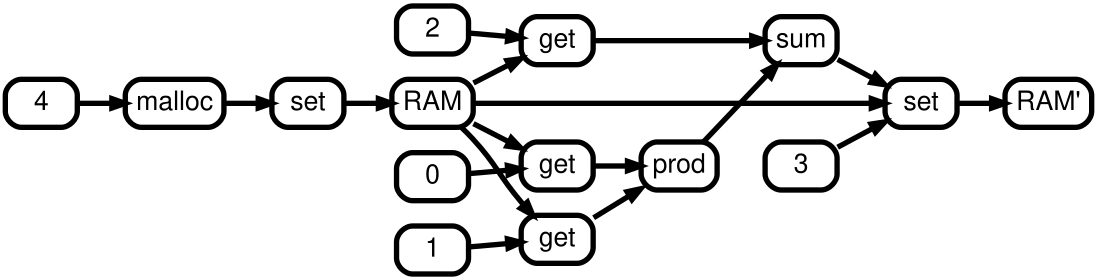
\includegraphics[scale=0.25]{rtd31}

\pagebreak\subsection*{2. Vector multiplication}

\begin{lstlisting}
A = malloc(4);
B = malloc(4);
C = malloc(4);
C[0] = A[0] * B[0];
C[1] = A[1] * B[1];
C[2] = A[2] * B[2];
C[3] = A[3] * B[3];
\end{lstlisting}

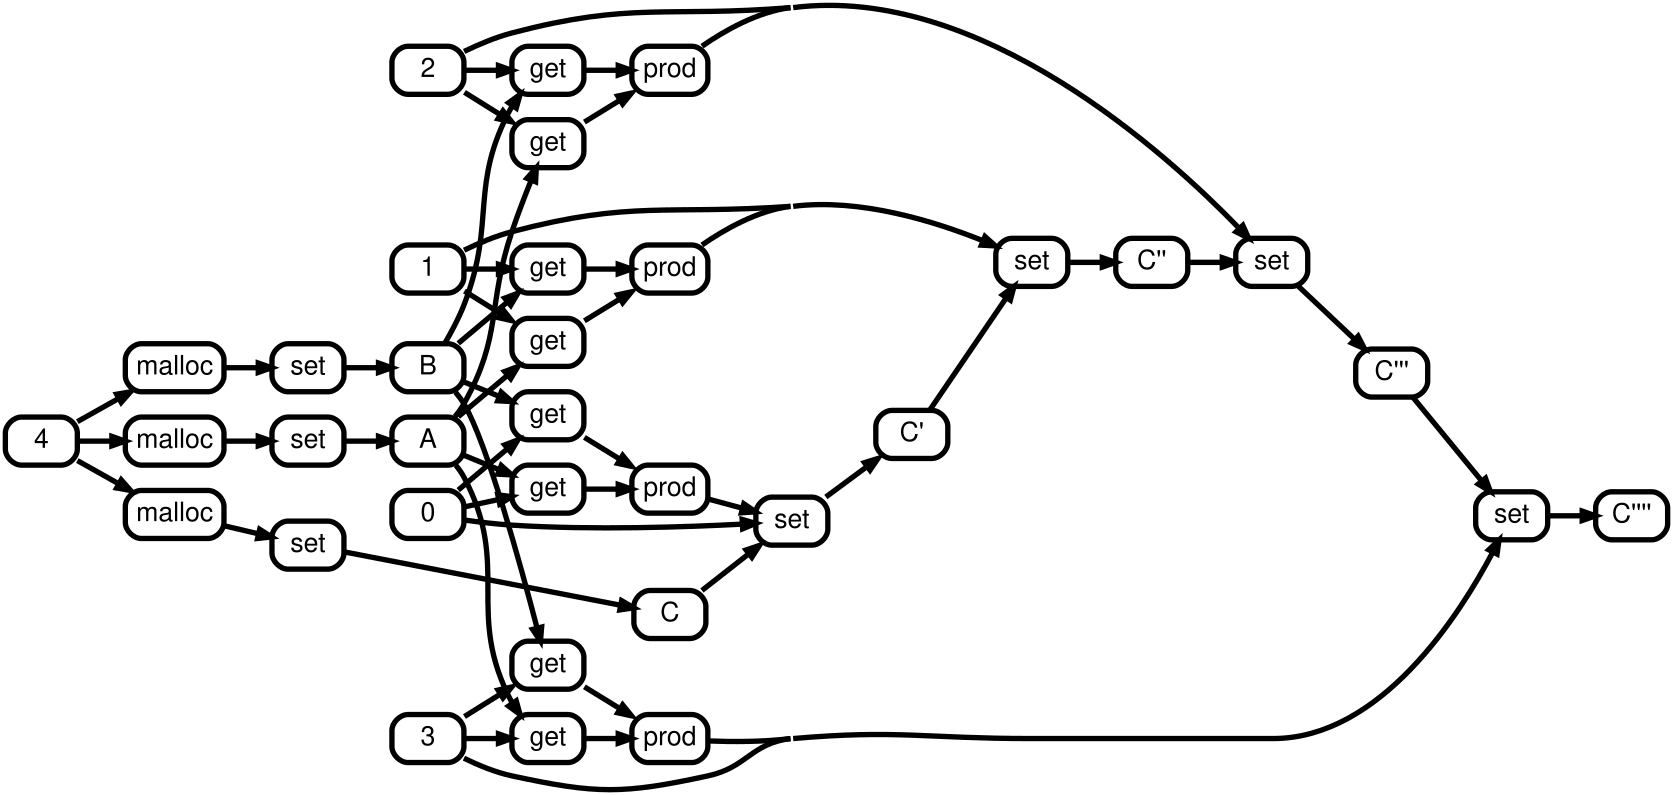
\includegraphics[scale=0.25]{rtd32}

\pagebreak\subsection*{3. Dot product}

\begin{lstlisting}
A = malloc(4);
B = malloc(4);
C = malloc(1);
C[0] = A[0] * B[0] +
       A[1] * B[1] +
       A[2] * B[2] +
       A[3] * B[3];
\end{lstlisting}

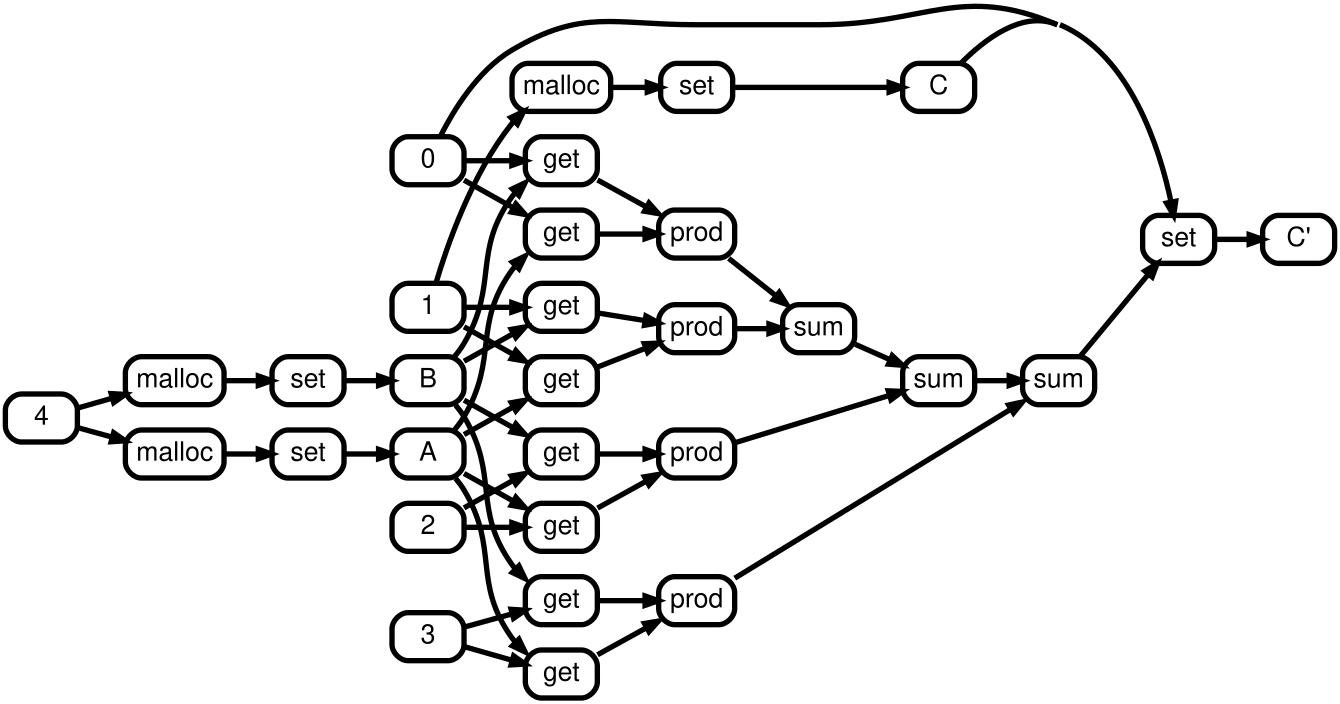
\includegraphics[scale=0.25]{rtd33}

\pagebreak\subsection*{4. Convolution}

\begin{lstlisting}
A = malloc(6);
W = malloc(3);
C = malloc(4);
C[0] = A[0] * W[0] + A[1] * W[1] + A[2] * W[2];
C[1] = A[1] * W[0] + A[2] * W[1] + A[3] * W[2];
C[2] = A[2] * W[0] + A[3] * W[1] + A[4] * W[2];
C[3] = A[3] * W[0] + A[4] * W[1] + A[5] * W[2];
\end{lstlisting}

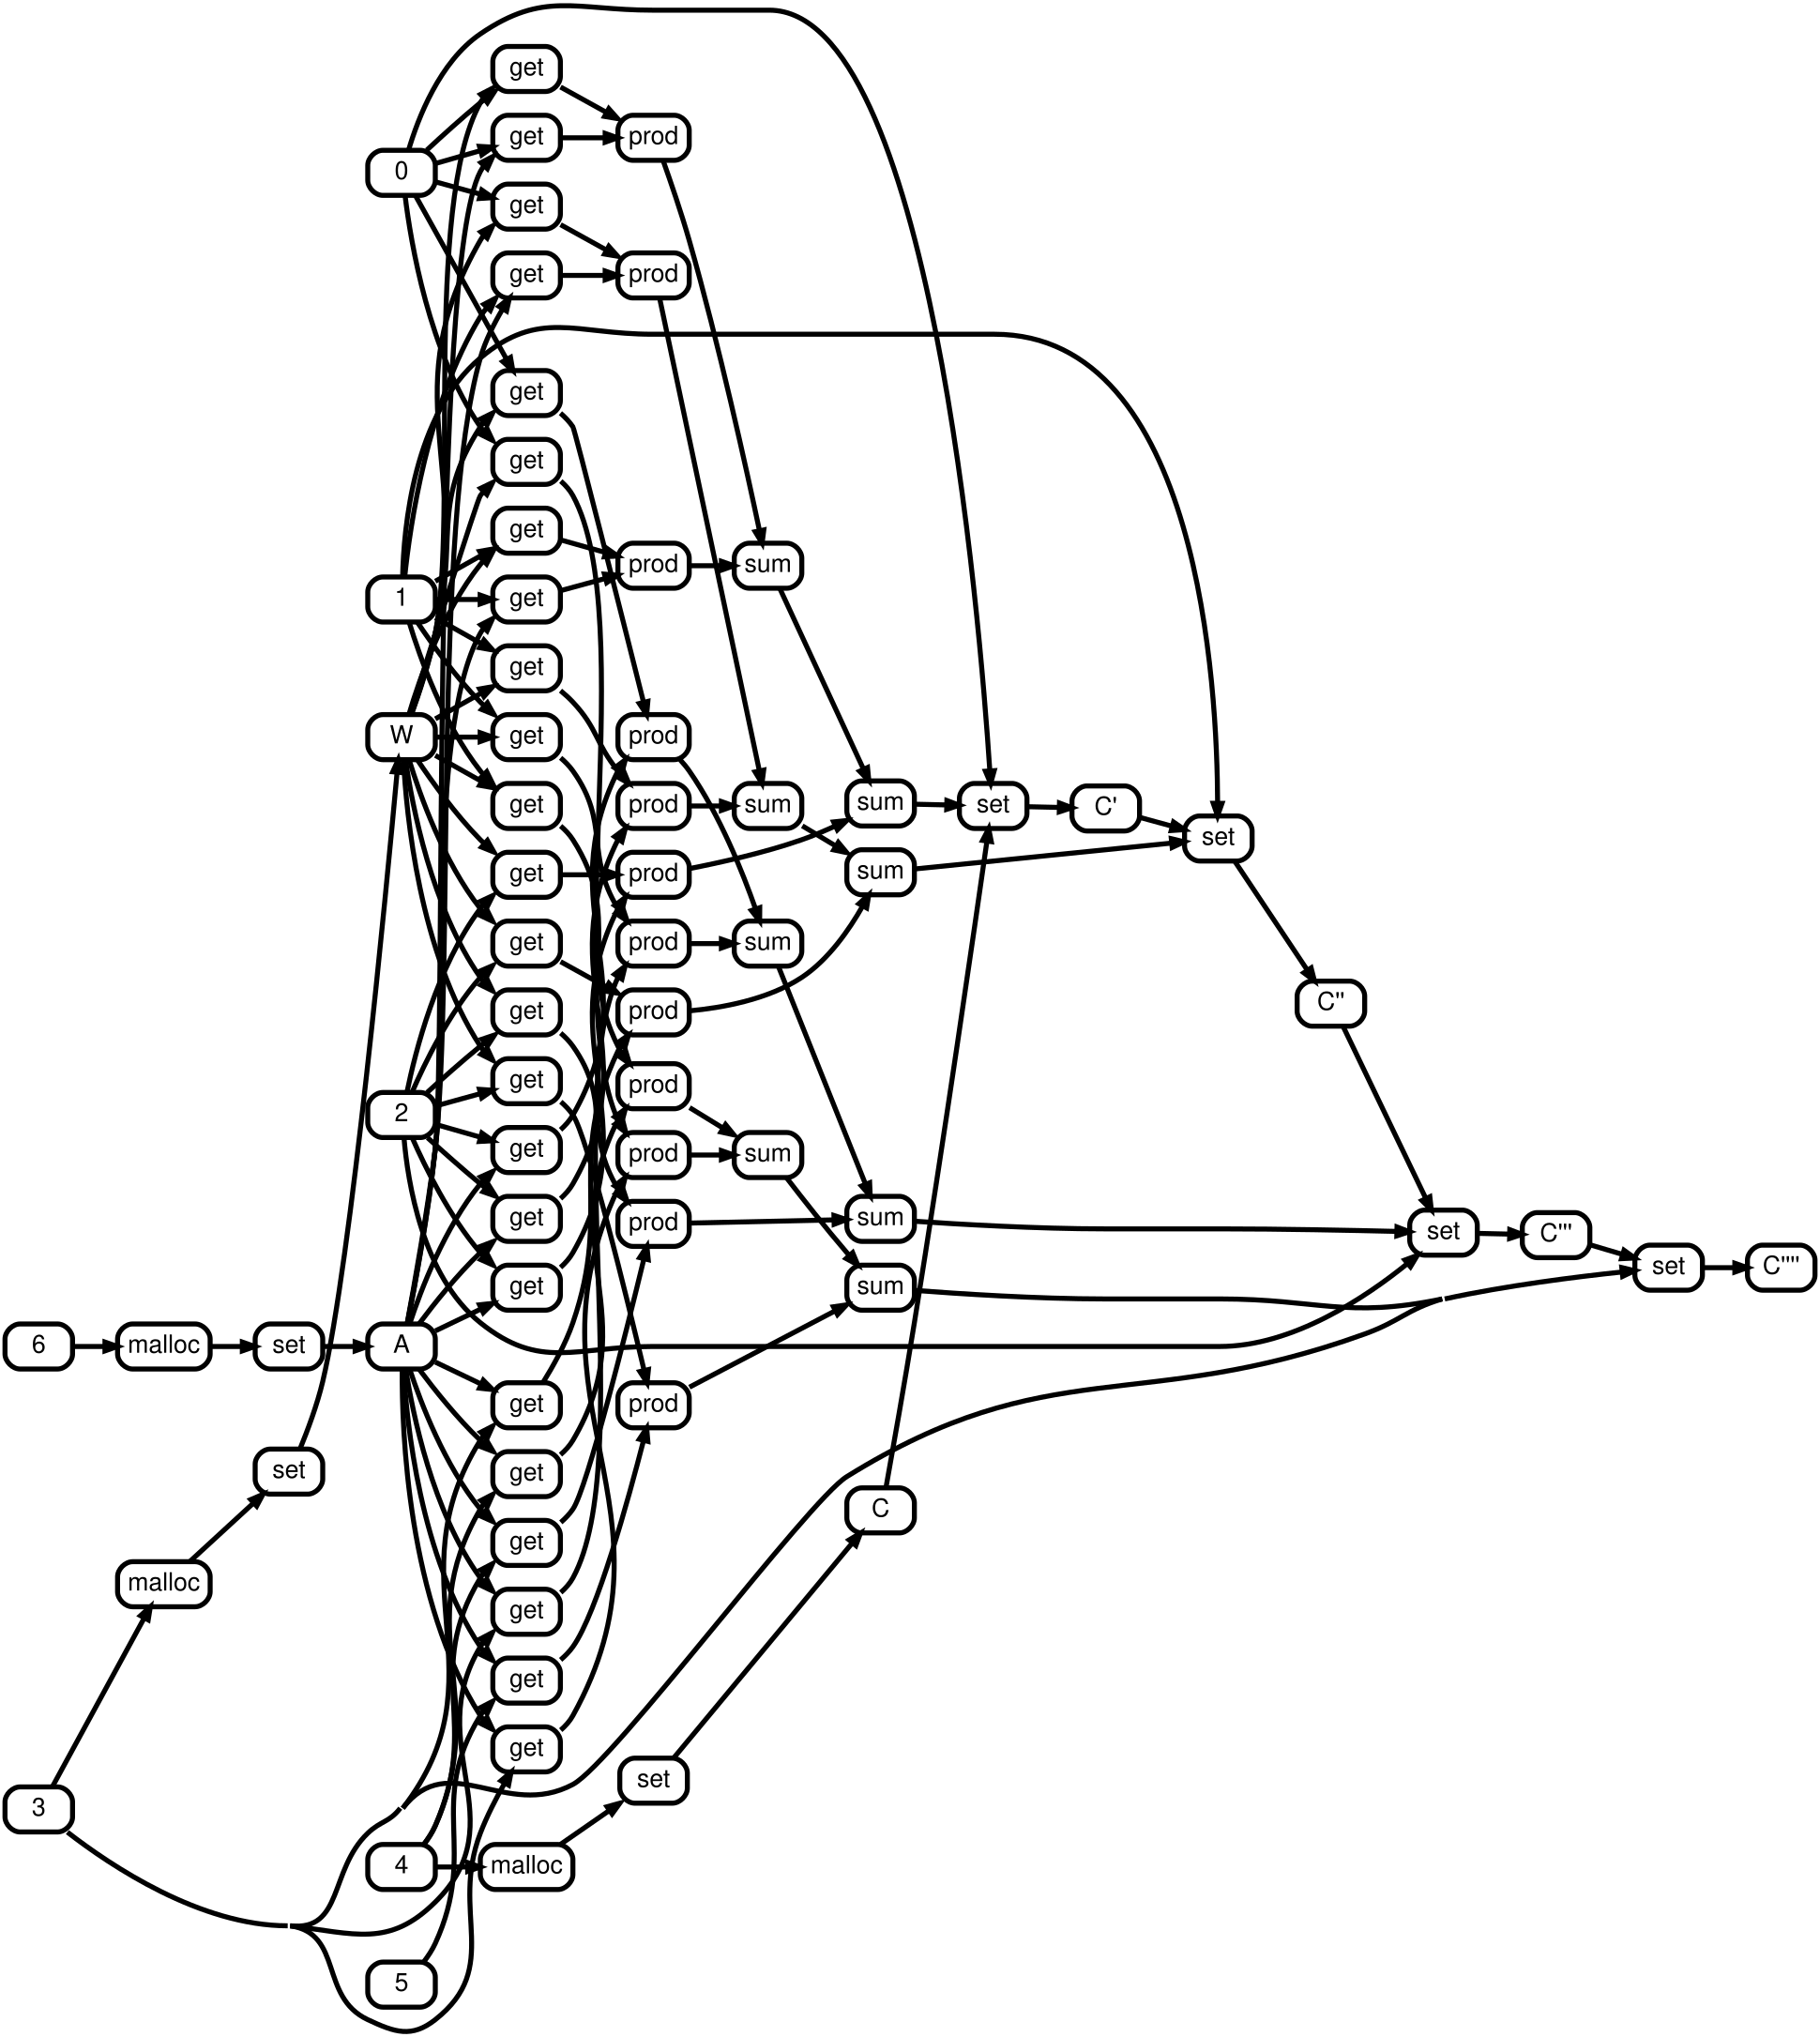
\includegraphics[scale=0.25]{rtd34}

\pagebreak\section*{IV. Extensions/Optimizations}

\subsection*{1. Simple variable test}

\begin{lstlisting}
I = 0;
I = 1;
I = I+J;
\end{lstlisting}

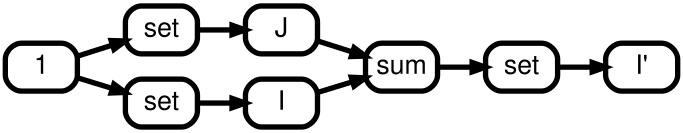
\includegraphics[scale=0.25]{rtd41}

\pagebreak\subsection*{2. Simple loop test}

\begin{lstlisting}
S = 0.w
for(i in 0..3) { // 4 iterations
    S = S + i.w
}
\end{lstlisting}

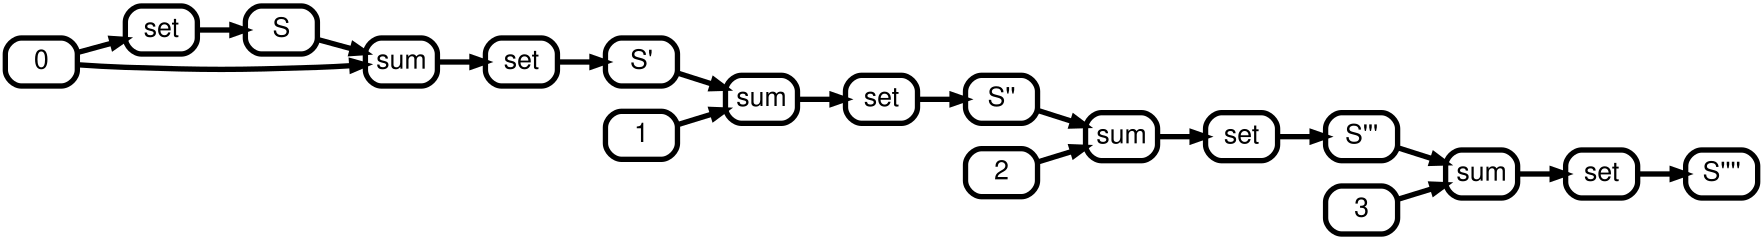
\includegraphics[scale=0.25]{rtd42}

\pagebreak\subsection*{3. Sum of array}

\begin{lstlisting}
A = malloc(4);
S = 0.w;
for (i in 0..3) { // 4 iterations
    S += A[i]
}
\end{lstlisting}

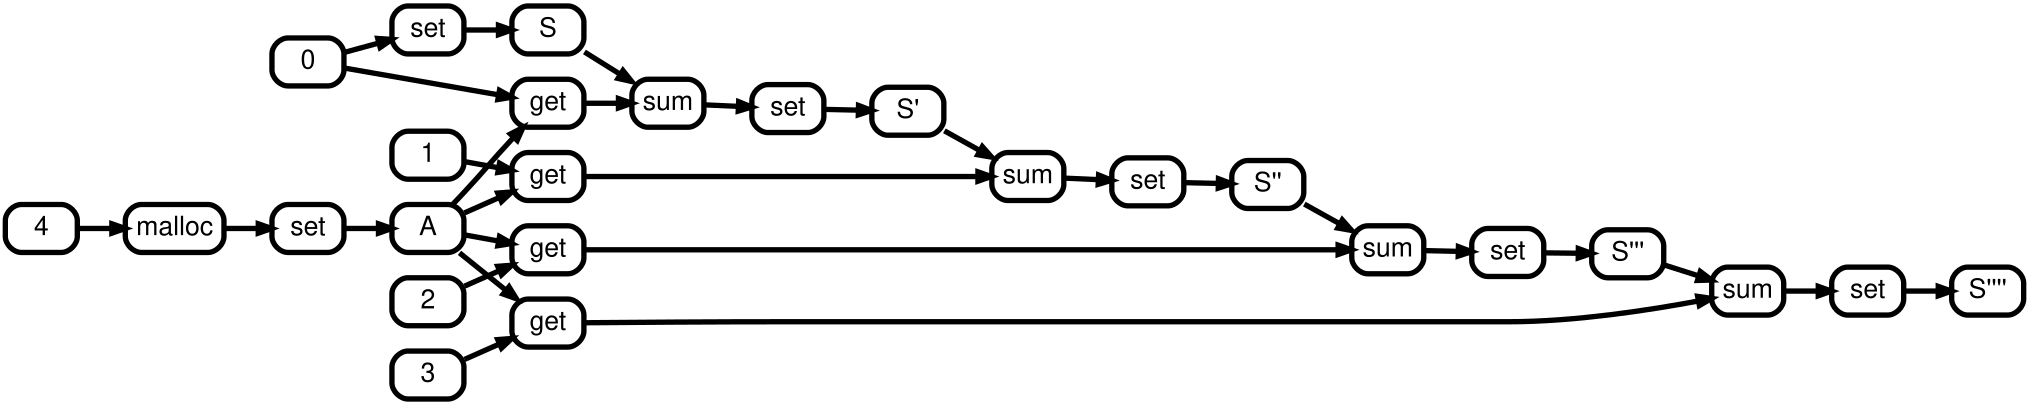
\includegraphics[scale=0.25]{rtd43}

\pagebreak\subsection*{4. Dot product}

\begin{lstlisting}
A = malloc(4);
B = malloc(4);
S = 0.w;
for (i in 0..3) { // 4 iterations
    S = S + A[i] * B[i];
}
\end{lstlisting}

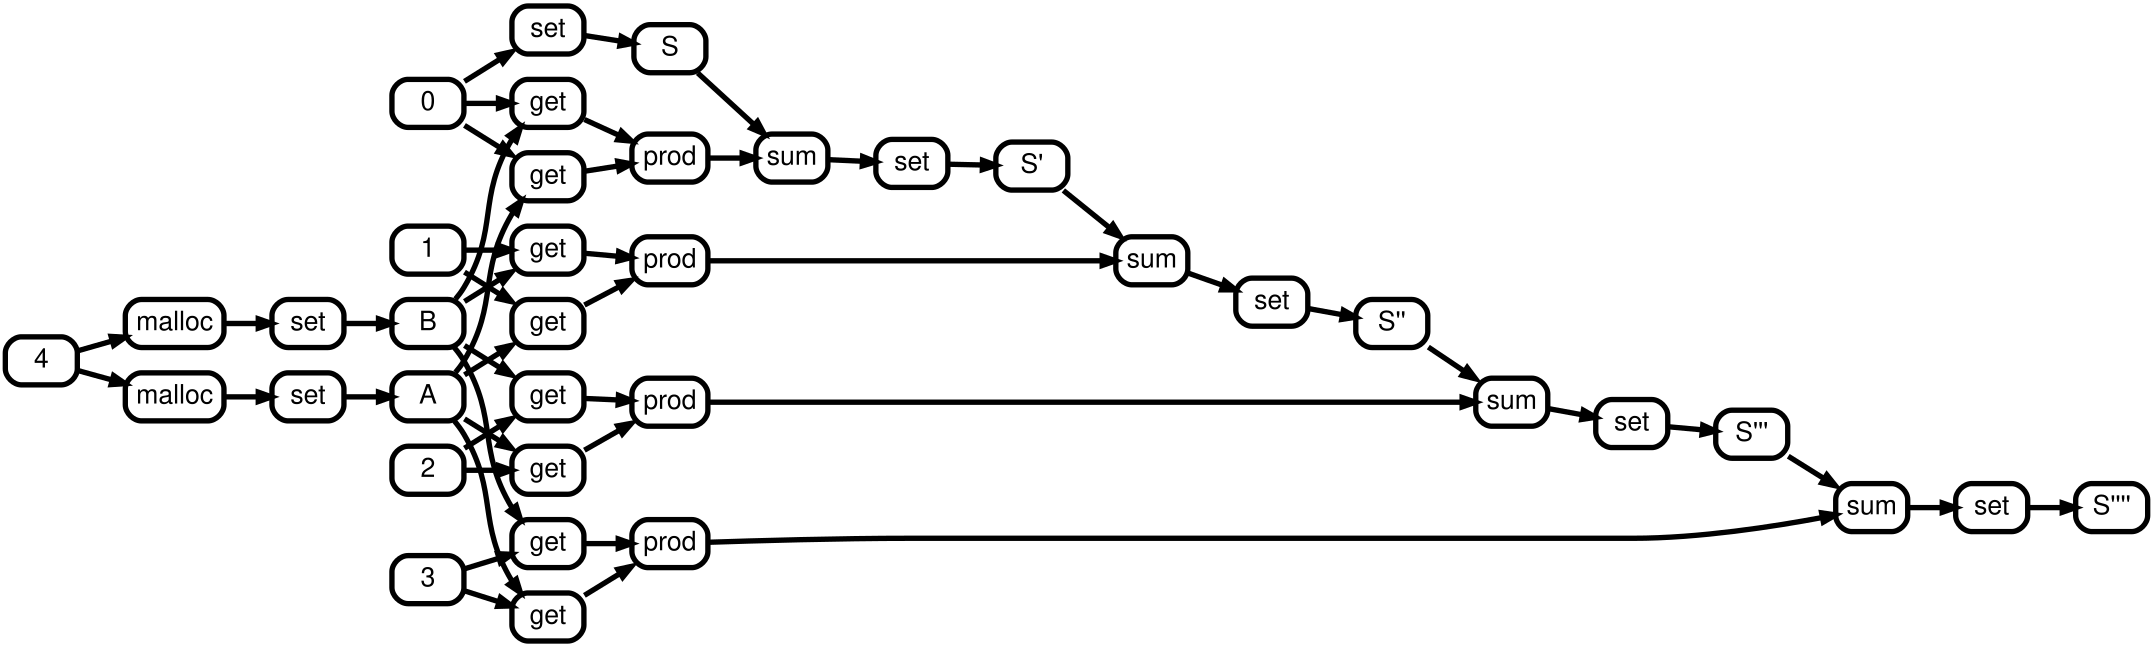
\includegraphics[scale=0.25]{rtd44}
\end{document}